\documentclass[10pt]{article}
\usepackage[margin=0.7in]{geometry}
\usepackage{amsmath,booktabs,graphicx,longtable,array}
\usepackage[T1]{fontenc}
\newcommand{\code}[1]{\texttt{#1}}
\title{Stationary profiles under four boundary couplings}
\author{Numerical audit report}
\date{2026-09-06}
\begin{document}
\maketitle

\section*{Frozen design}
The corrected SIMD implementation evolves 16 trajectories per batch with
$\gamma=0.1$, maximum $dt=5\times10^{-4}$, and corrected noises
$\sigma_I=2\sqrt{2\gamma T I}$ and
$\sigma_\phi=\sqrt{2\gamma T/I}$.  The four couplings are
BC1 $(b_I,b_\phi)=(2\gamma(2T-F),\gamma P)$,
BC2 $(2\gamma(2T-F),0)$,
BC3 $(2\gamma(2T-I^2),0)$, and
BC3b $(2\gamma(2T-I^2),\gamma P)$.
Here $F=2MI_1-I_1^2+2I_1I_2\cos\delta$ and
$P=2I_2\sin\delta$, with the reflected right-boundary expression.
The run matrix contains 36 logical conditions, each formed from two fixed seeds
and 512 trajectories. Burn-ins are 2000, 8000, and 32000 for
$n=25,50,100$; all measurement durations are 2000.

\section*{BC1 reproduction gate}
\begin{center}\small
\begin{tabular}{rrrllll}
\toprule
$n$ & side & reference & new mean $\pm$ SE & difference & tolerance & verdict\\
\midrule
25 & left & 0.737907 & 0.73727 $\pm$ 0.000599 & -0.000637 & 0.0148 & PASS \\
25 & right & 0.165409 & 0.1652941 $\pm$ 0.000168 & -0.000115 & 0.00331 & PASS \\
50 & left & 0.514213 & 0.5169271 $\pm$ 0.000711 & 0.00271 & 0.0103 & PASS \\
50 & right & 0.105599 & 0.1063664 $\pm$ 0.000156 & 0.000767 & 0.00211 & PASS \\
100 & left & 0.361686 & 0.3582186 $\pm$ 0.000858 & -0.00347 & 0.00723 & PASS \\
100 & right & 0.0728212 & 0.07204994 $\pm$ 0.000178 & -0.000771 & 0.002 & PASS \\
\bottomrule
\end{tabular}
\end{center}

\section*{Profiles}
Shaded bands are pointwise 95\% intervals across independent trajectory time
averages.  Every per-site numerical value is in the accompanying merged CSV.
\begin{figure}[ht]\centering
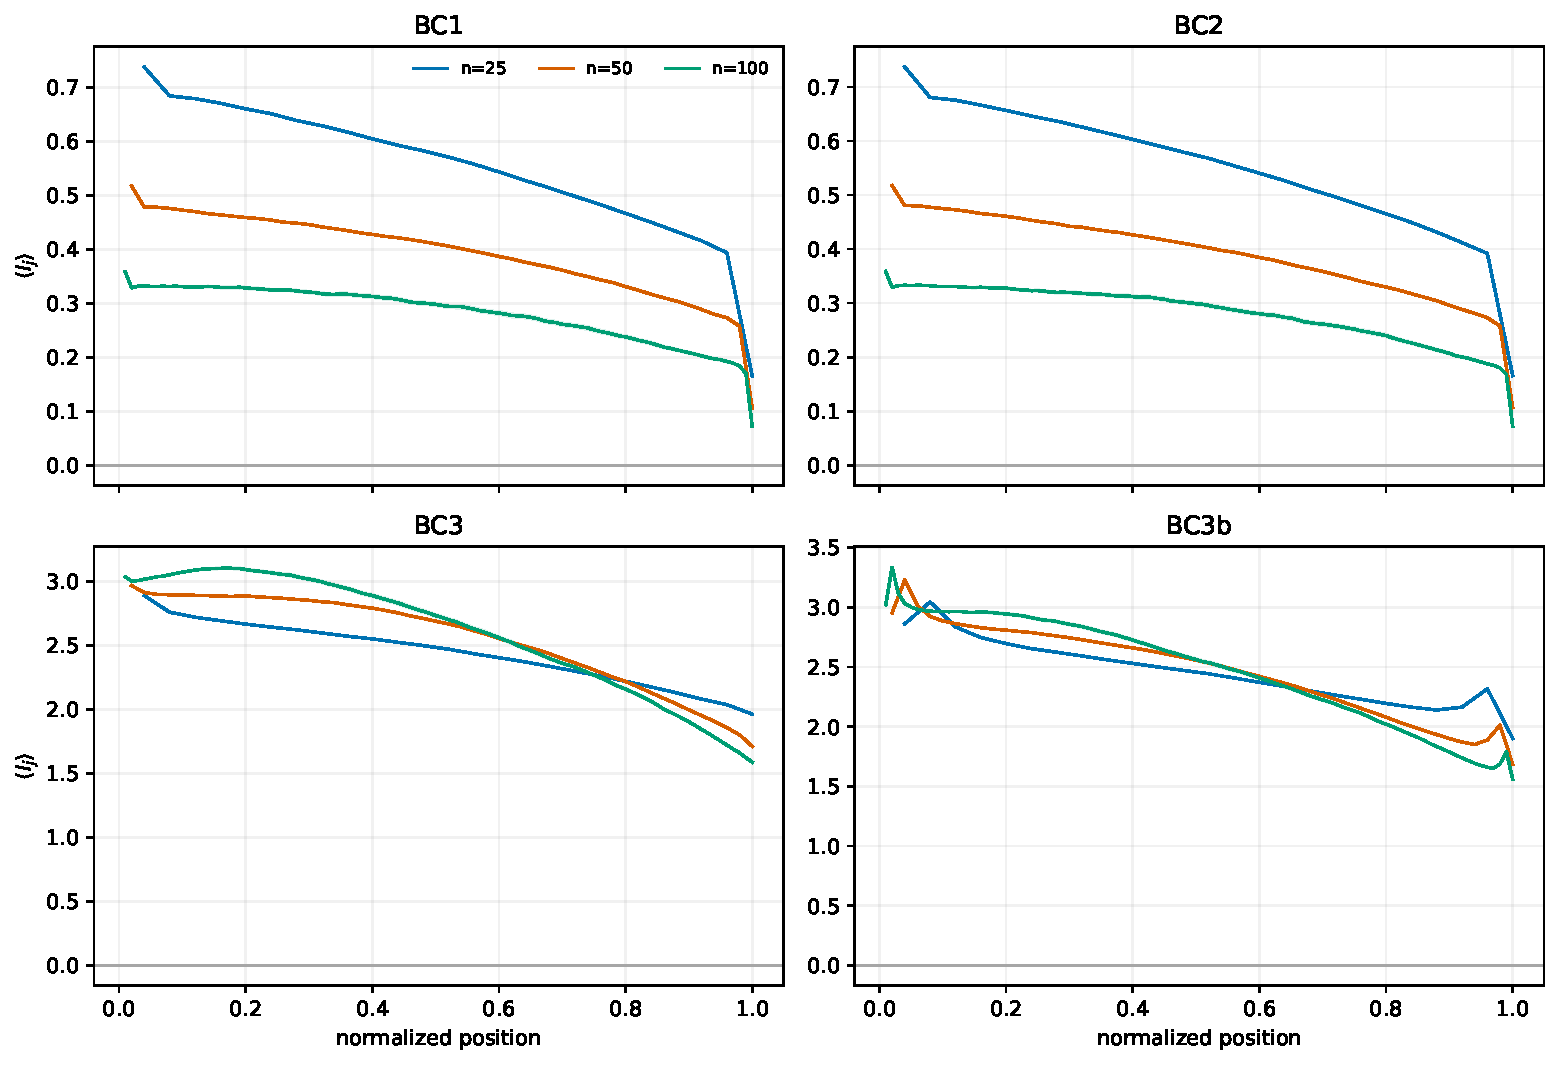
\includegraphics[width=0.98\textwidth]{../figures/action_profiles_T10_T2.pdf}
\caption{Action profiles for $(T_1,T_n)=(10,2)$.}\end{figure}
\begin{figure}[ht]\centering
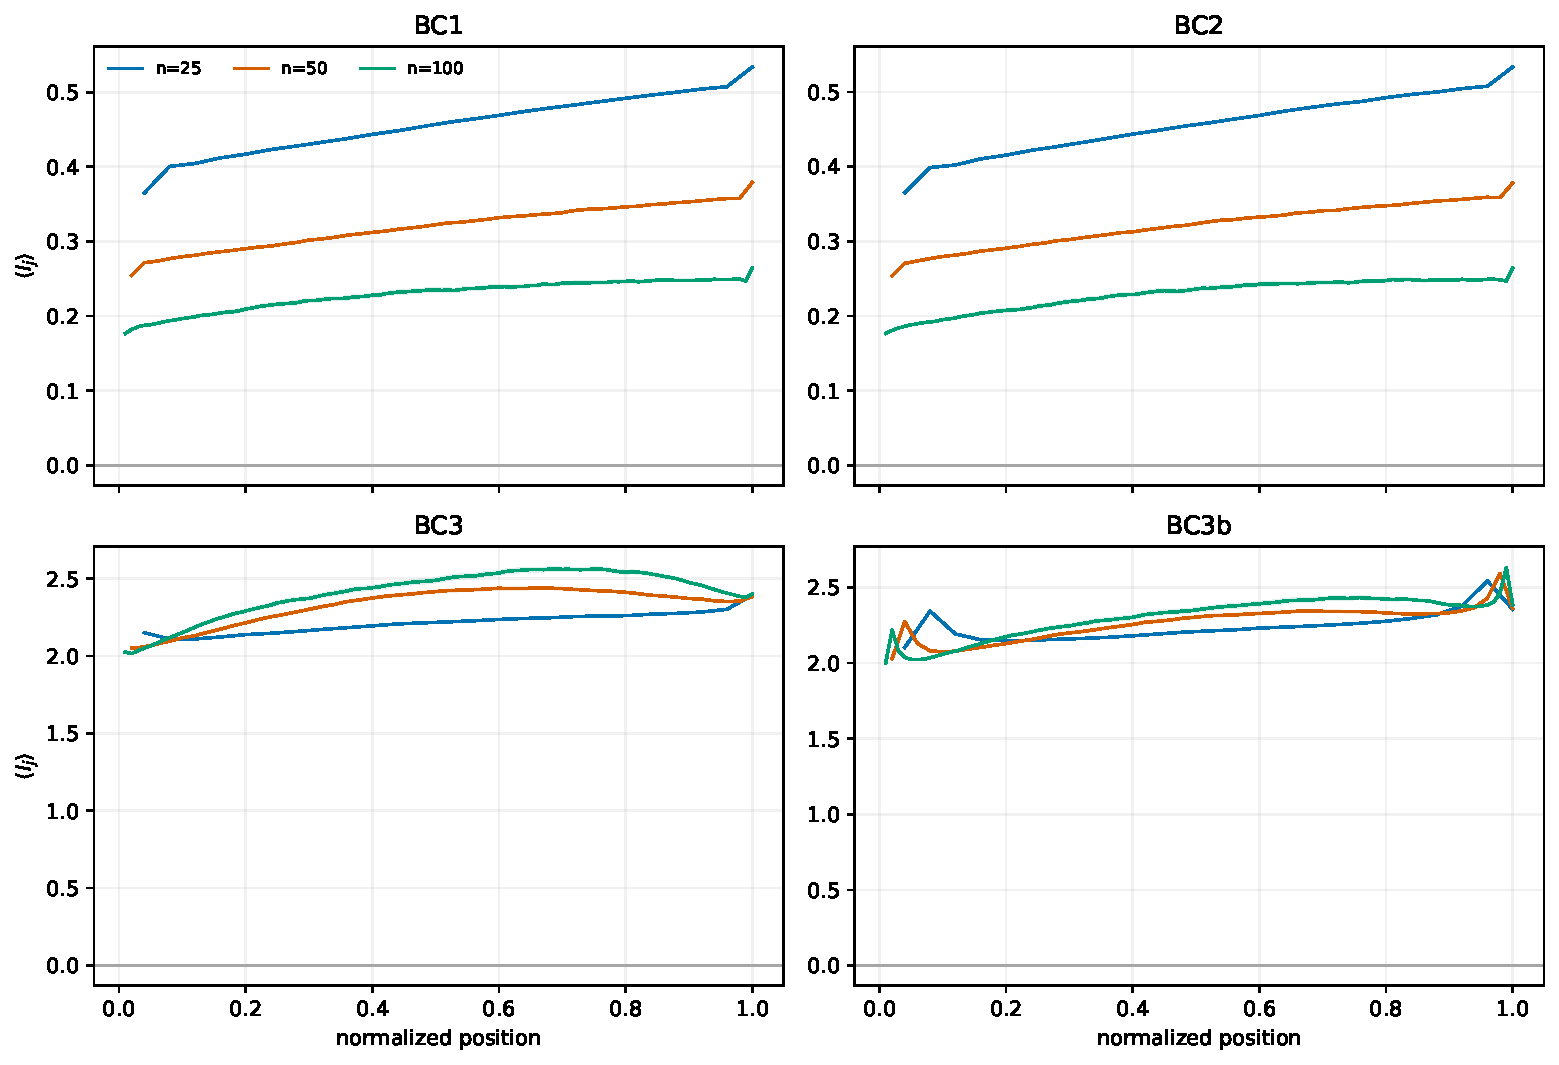
\includegraphics[width=0.98\textwidth]{../figures/action_profiles_T4_T6.pdf}
\caption{Action profiles for $(T_1,T_n)=(4,6)$.}\end{figure}
\begin{figure}[ht]\centering
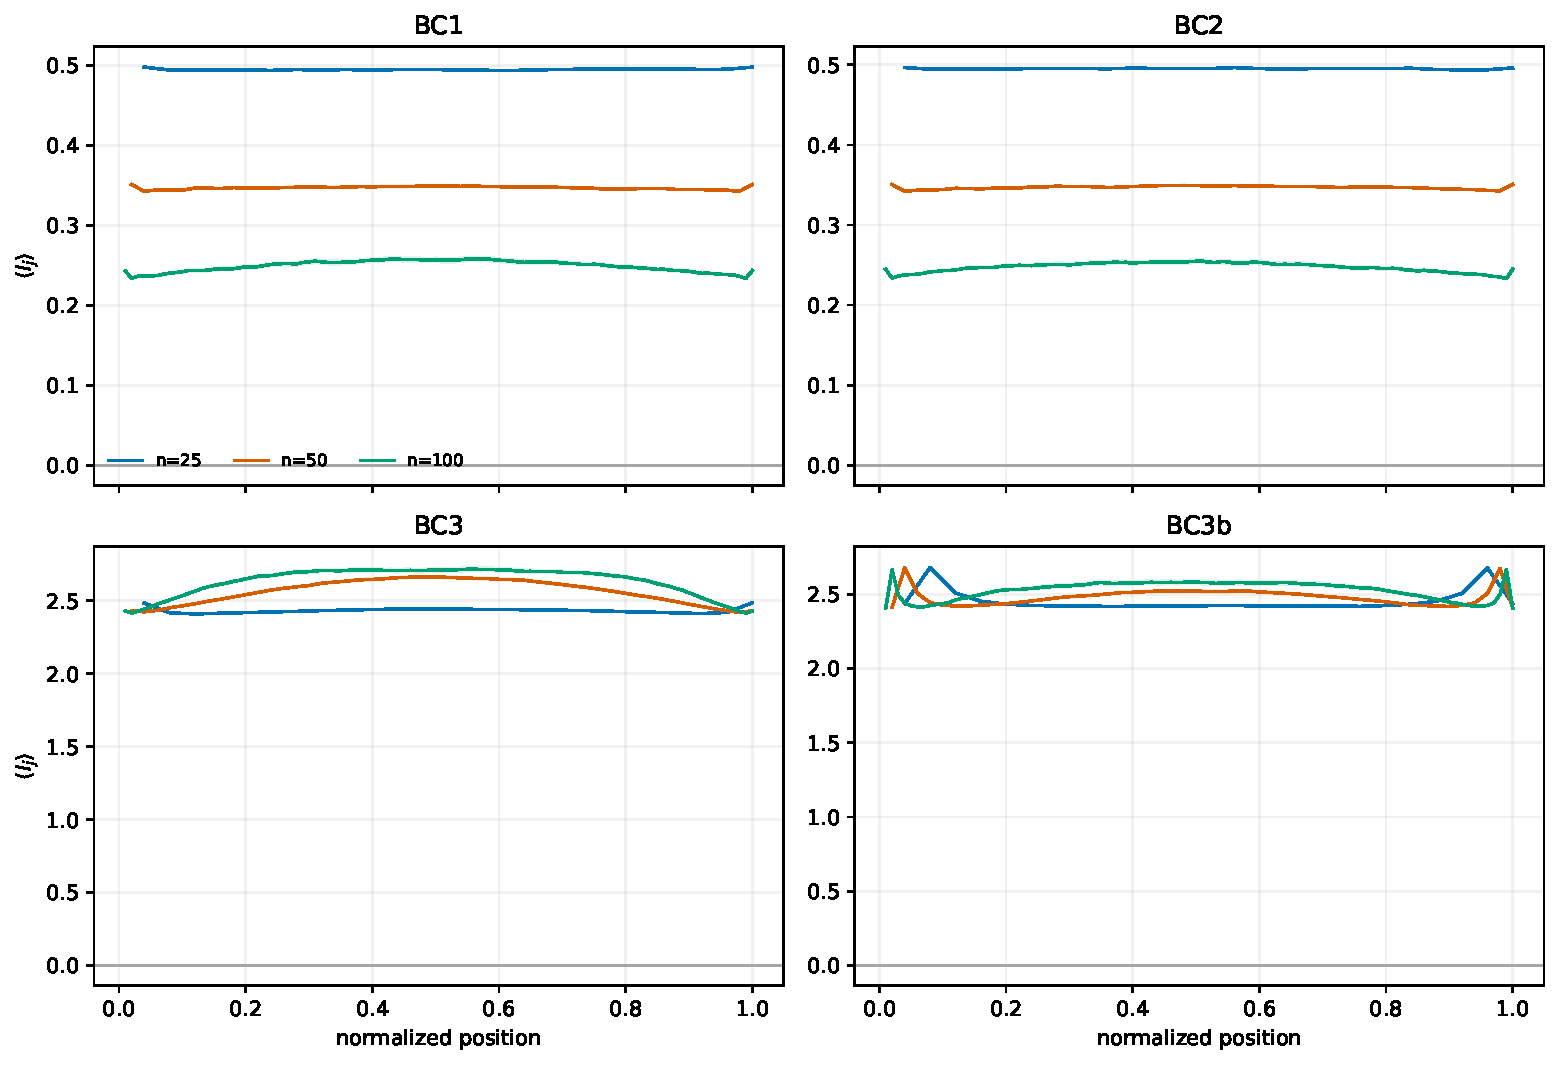
\includegraphics[width=0.98\textwidth]{../figures/action_profiles_T6_T6.pdf}
\caption{Equal-temperature action profiles.}\end{figure}
\begin{figure}[ht]\centering
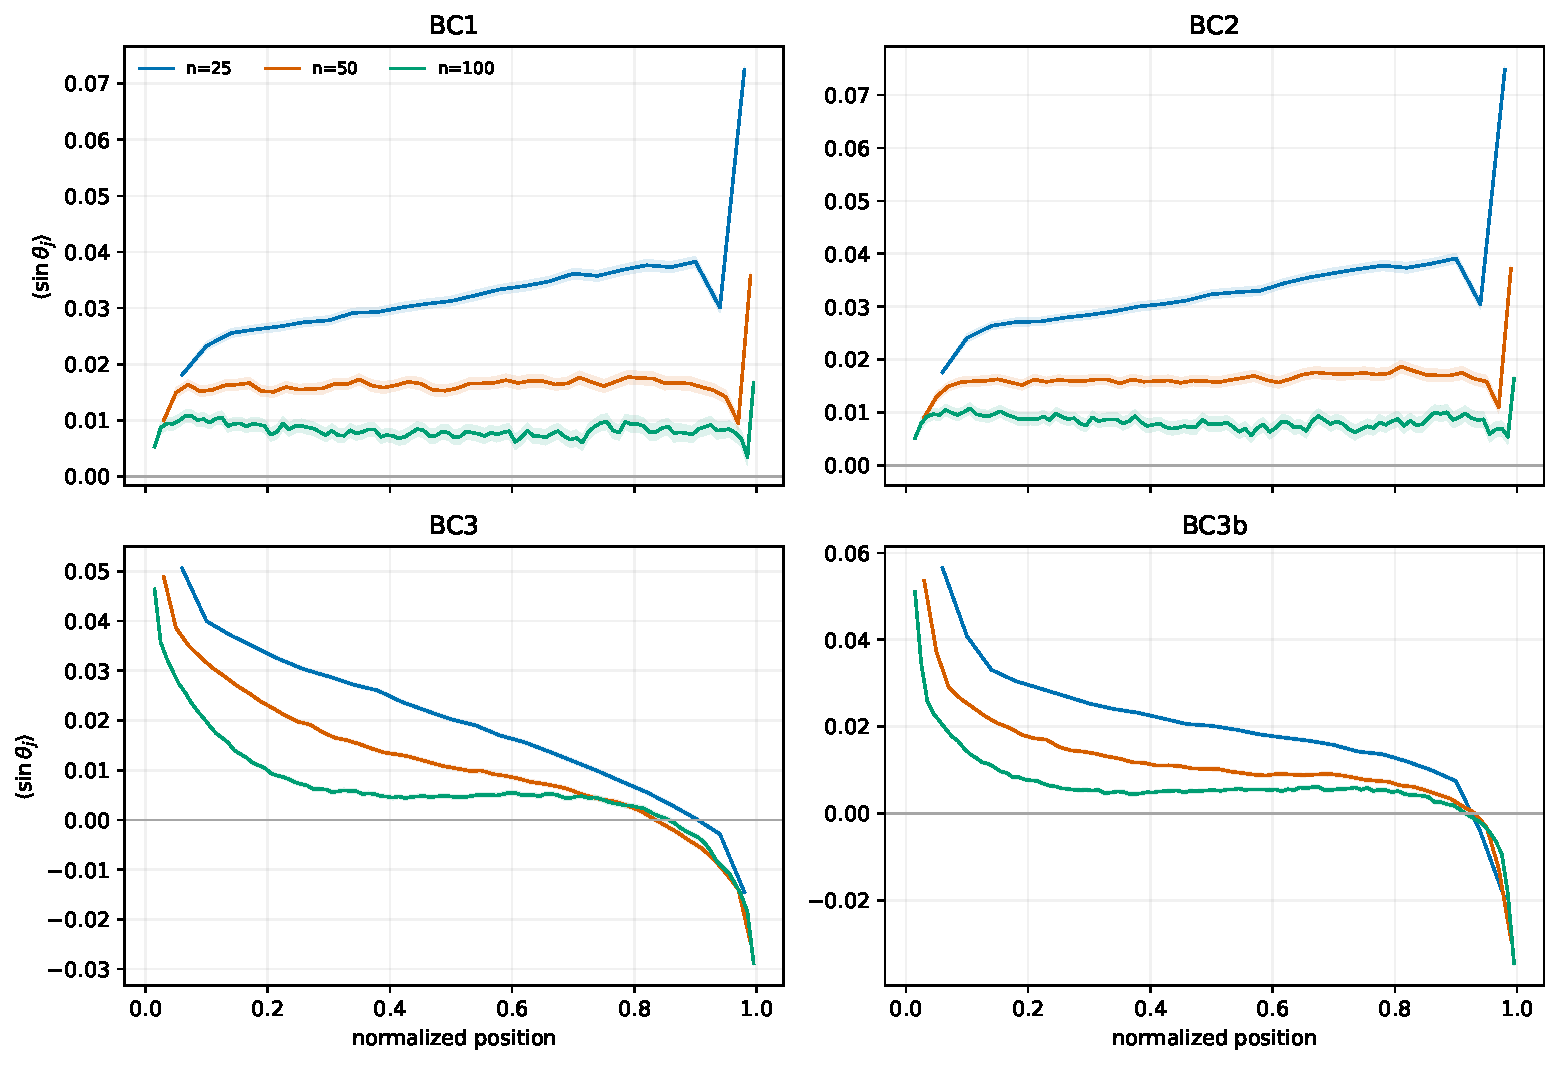
\includegraphics[width=0.98\textwidth]{../figures/sine_profiles_T10_T2.pdf}
\caption{Bond-sine profiles for $(T_1,T_n)=(10,2)$.}\end{figure}
\begin{figure}[ht]\centering
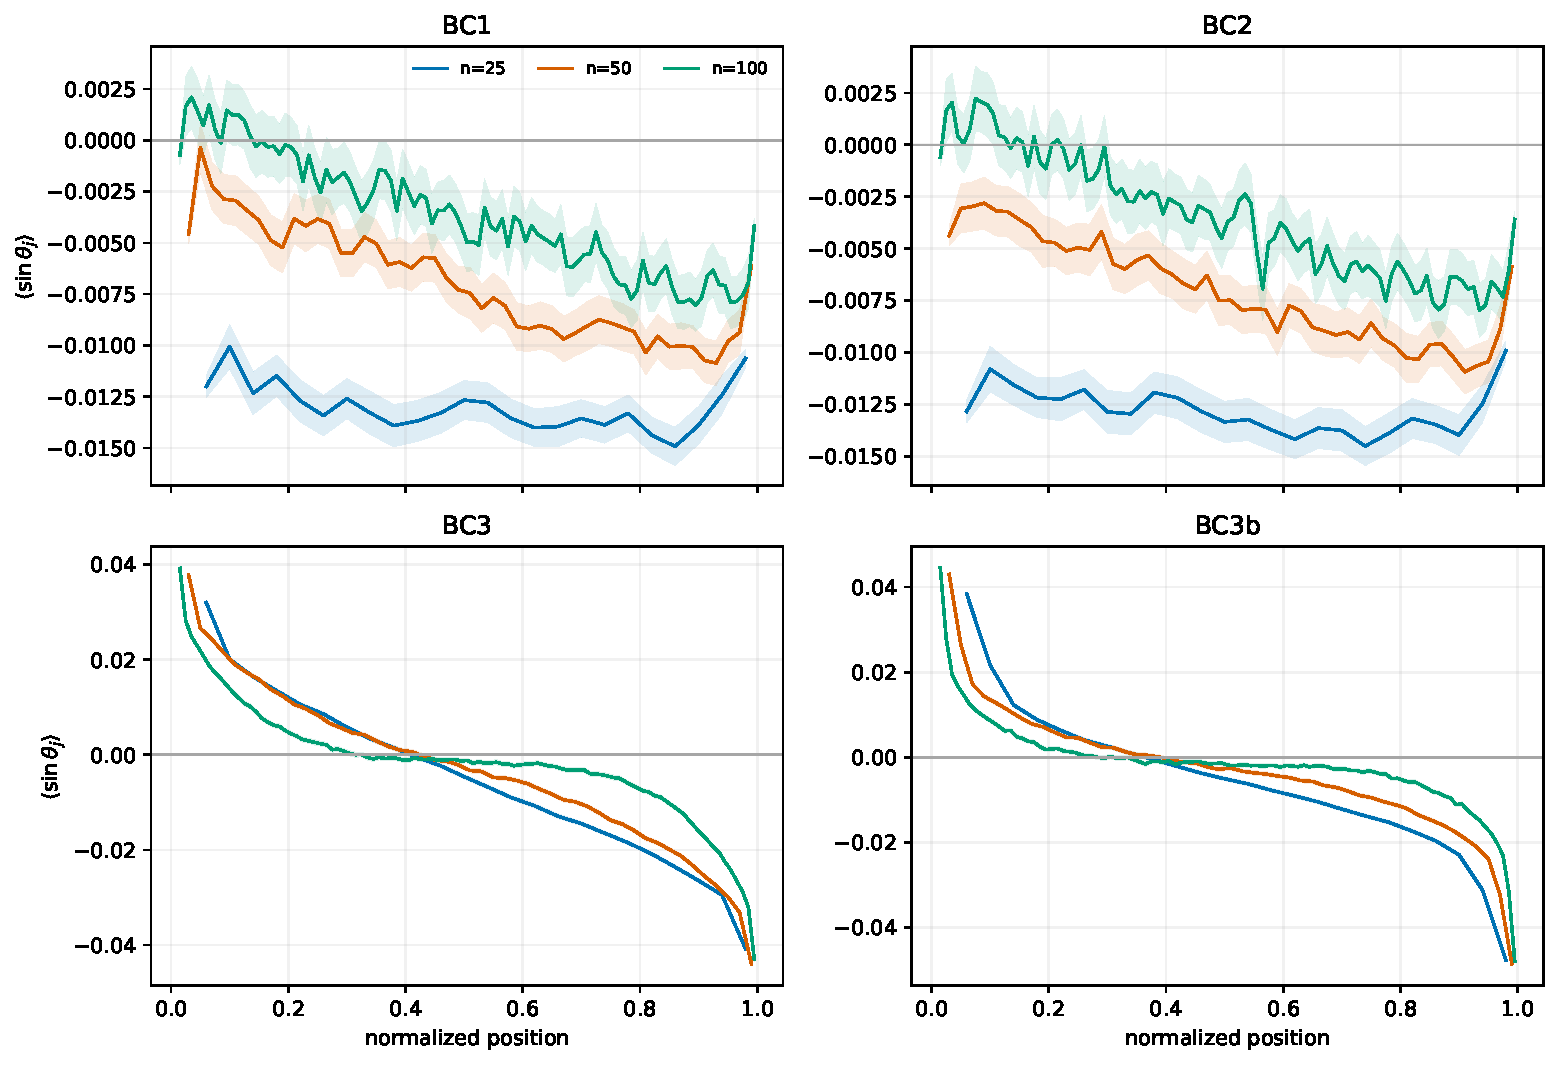
\includegraphics[width=0.98\textwidth]{../figures/sine_profiles_T4_T6.pdf}
\caption{Bond-sine profiles for $(T_1,T_n)=(4,6)$.}\end{figure}
\begin{figure}[ht]\centering
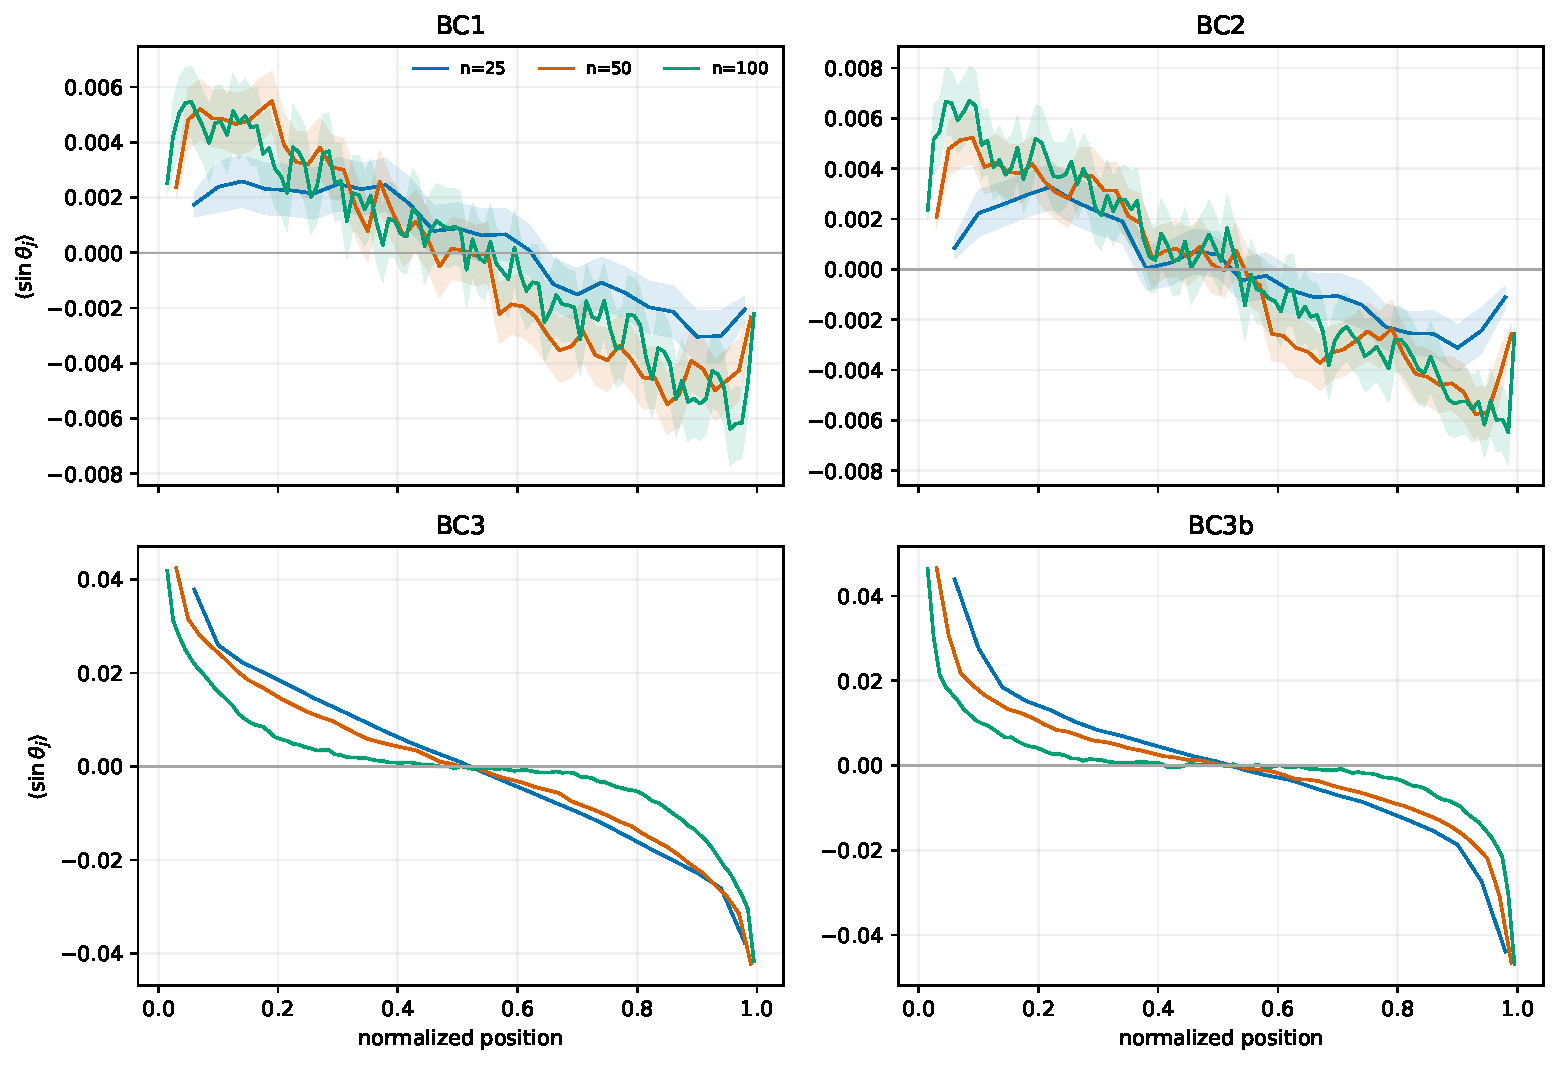
\includegraphics[width=0.98\textwidth]{../figures/sine_profiles_T6_T6.pdf}
\caption{Equal-temperature bond-sine profiles.}\end{figure}

\clearpage
\section*{Equal-temperature control}
The action columns report the spatial mean and relative range.  ``Sine 95\%
failures'' counts individual bonds outside a pointwise interval; the simultaneous
verdict uses a Bonferroni 95\% threshold across all bonds and is not tuned by
case.
\begin{center}\small
\begin{tabular}{lrrrrrl}
\toprule BC & $n$ & mean $I$ & relative range & sine 95\% failures & max $|z|$ & simultaneous sine\\
\midrule
BC1 & 25 & 0.4947 & 0.00894 & 19 & 8.68 & FAIL \\
BC1 & 50 & 0.3468 & 0.0238 & 40 & 11.6 & FAIL \\
BC1 & 100 & 0.2492 & 0.0973 & 71 & 12.9 & FAIL \\
BC2 & 25 & 0.4951 & 0.0057 & 17 & 7.07 & FAIL \\
BC2 & 50 & 0.3469 & 0.0241 & 39 & 12.6 & FAIL \\
BC2 & 100 & 0.2474 & 0.0881 & 78 & 13 & FAIL \\
BC3 & 25 & 2.434 & 0.0312 & 24 & 210 & FAIL \\
BC3 & 50 & 2.564 & 0.0945 & 47 & 244 & FAIL \\
BC3 & 100 & 2.636 & 0.114 & 87 & 232 & FAIL \\
BC3b & 25 & 2.454 & 0.107 & 24 & 233 & FAIL \\
BC3b & 50 & 2.481 & 0.108 & 47 & 266 & FAIL \\
BC3b & 100 & 2.528 & 0.103 & 77 & 254 & FAIL \\
\bottomrule\end{tabular}\end{center}

\section*{Central-profile scaling}
The exponent is the unconstrained three-point OLS slope of
$\log\langle I\rangle_{\rm mid}$ against $\log n$.  The quoted standard error
has one residual degree of freedom and must not be read as an asymptotic
confidence interval.
\begin{figure}[ht]\centering
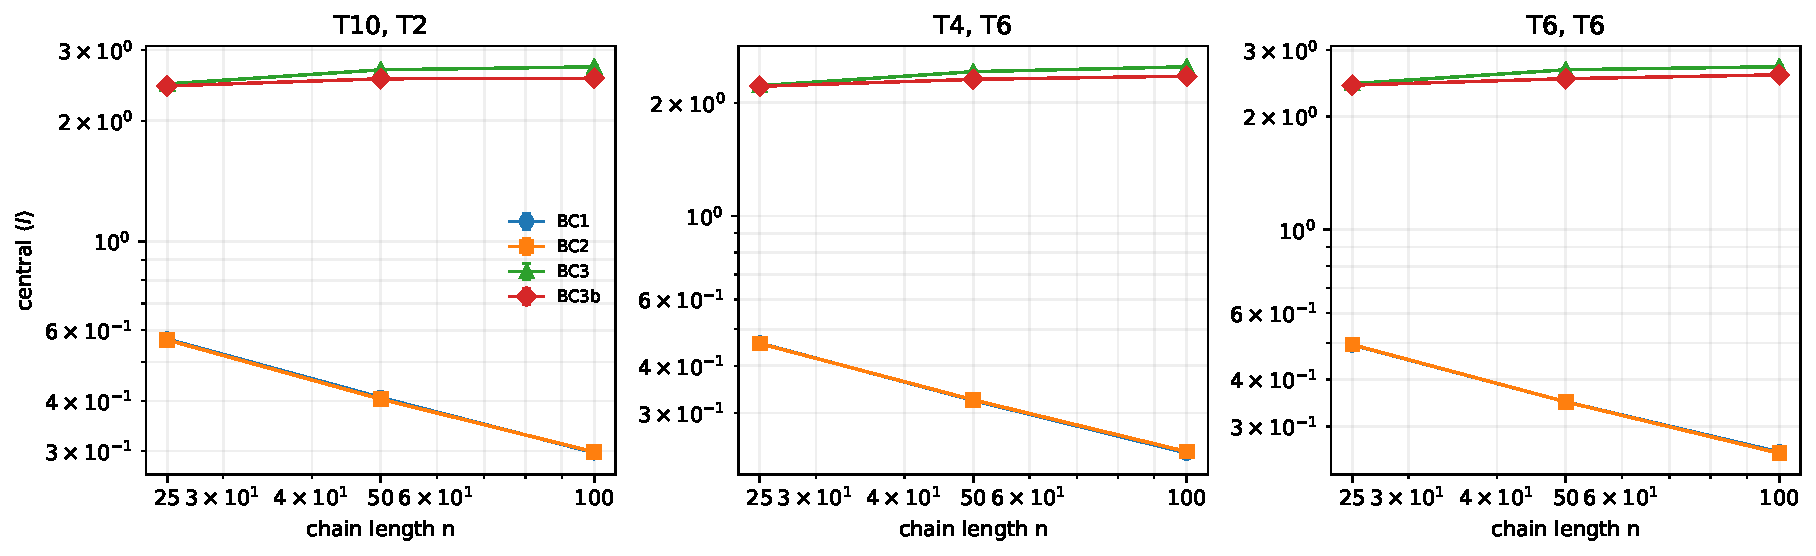
\includegraphics[width=0.98\textwidth]{../figures/midpoint_scaling.pdf}
\caption{Central action versus chain length.}\end{figure}
\begin{center}\scriptsize
\begin{tabular}{llrrrr}
\toprule BC & temperatures & slope $\pm$ SE & $R^2$ & reference & values at 25;50;100\\
\midrule
BC1 & T10\_T2 & -0.4709 $\pm$ 0.0077 & 1 & -0.5 & 0.57075641472457761;0.40800609000054661;0.29711230508365449 \\
BC1 & T4\_T6 & -0.485 $\pm$ 0.012 & 0.999 & -0.5 & 0.4595982885930664;0.32366108783401182;0.23461799285221979 \\
BC1 & T6\_T6 & -0.4728 $\pm$ 0.017 & 0.999 & -0.5 & 0.49427130751800652;0.34893647316394089;0.25662486999643297 \\
BC2 & T10\_T2 & -0.464 $\pm$ 0.015 & 0.999 & -0.5 & 0.56782804383747676;0.40437215110819974;0.29846292921079032 \\
BC2 & T4\_T6 & -0.4772 $\pm$ 0.012 & 0.999 & -0.5 & 0.45848748914233373;0.32480221074059445;0.23659502395181325 \\
BC2 & T6\_T6 & -0.4794 $\pm$ 0.015 & 0.999 & -0.5 & 0.495119447241124;0.34891066499724782;0.25471847277637671 \\
BC3 & T10\_T2 & 0.07078 $\pm$ 0.026 & 0.877 & 0 & 2.471247624778929;2.6793568958950607;2.7260360316502132 \\
BC3 & T4\_T6 & 0.08346 $\pm$ 0.023 & 0.927 & 0 & 2.2210690330063083;2.4202429589373065;2.493496764643881 \\
BC3 & T6\_T6 & 0.07498 $\pm$ 0.028 & 0.881 & 0 & 2.4447472518854778;2.6616374138955017;2.7125569429313616 \\
BC3b & T10\_T2 & 0.03203 $\pm$ 0.016 & 0.808 & 0 & 2.4426077420024015;2.5447156133283504;2.5535220530397358 \\
BC3b & T4\_T6 & 0.04487 $\pm$ 0.0094 & 0.958 & 0 & 2.213014281135564;2.3087251556346784;2.3550359591268659 \\
BC3b & T6\_T6 & 0.04554 $\pm$ 0.0063 & 0.981 & 0 & 2.4232141576449502;2.5200353533441842;2.5811460396663919 \\
\bottomrule\end{tabular}\end{center}

\clearpage
\section*{Stability and reproducibility}
Endpoint changes compare the cumulative profile at 75\% and 100\% of the
fixed measurement interval.  Seed $z_{\max}$ is the largest pointwise
replicate difference divided by its independent-replicate SE over all sites and
bonds; all individual values remain available in the CSVs.
\begin{longtable}{lllrrrrrr}
\toprule BC & temperatures & $n$ & nonfinite & discarded & projections & seed $z_{\max}$ & left change & right change\\
\midrule\endfirsthead
\toprule BC & temperatures & $n$ & nonfinite & discarded & projections & seed $z_{\max}$ & left change & right change\\
\midrule\endhead
BC1 & T10\_T2 & 25 & 0 & 0 & 7879211 & 2.04 & 0.00181 & 0.000841 \\
BC1 & T10\_T2 & 50 & 0 & 0 & 28486375 & 2.55 & 5.95e-05 & 0.0005 \\
BC1 & T10\_T2 & 100 & 0 & 0 & 139662332 & 2.58 & -0.000145 & -0.000156 \\
BC1 & T4\_T6 & 25 & 0 & 0 & 6621345 & 1.9 & -0.000409 & -0.000272 \\
BC1 & T4\_T6 & 50 & 0 & 0 & 23412028 & 3 & -0.000773 & -0.0006 \\
BC1 & T4\_T6 & 100 & 0 & 0 & 113653924 & 3.61 & -9.25e-06 & 0.000201 \\
BC1 & T6\_T6 & 25 & 0 & 0 & 7178037 & 2.5 & -1.41e-05 & -0.000283 \\
BC1 & T6\_T6 & 50 & 0 & 0 & 25362163 & 2.62 & 0.000257 & 2.6e-06 \\
BC1 & T6\_T6 & 100 & 0 & 0 & 122987673 & 2.63 & 0.00125 & 0.000588 \\
BC2 & T10\_T2 & 25 & 0 & 0 & 7852119 & 2.17 & 0.000552 & 0.00029 \\
BC2 & T10\_T2 & 50 & 0 & 0 & 28428108 & 2.33 & 0.000339 & 0.000511 \\
BC2 & T10\_T2 & 100 & 0 & 0 & 139278800 & 2.96 & -0.000873 & -0.000489 \\
BC2 & T4\_T6 & 25 & 0 & 0 & 6616632 & 2.55 & -3.19e-05 & -0.000181 \\
BC2 & T4\_T6 & 50 & 0 & 0 & 23410693 & 2.52 & 0.00144 & 0.00123 \\
BC2 & T4\_T6 & 100 & 0 & 0 & 113642508 & 2.69 & -0.000517 & -0.00105 \\
BC2 & T6\_T6 & 25 & 0 & 0 & 7188374 & 2.38 & -7.89e-05 & -0.000344 \\
BC2 & T6\_T6 & 50 & 0 & 0 & 25329850 & 3.64 & 0.000693 & 0.000373 \\
BC2 & T6\_T6 & 100 & 0 & 0 & 122838383 & 3.46 & -0.00106 & -0.00124 \\
BC3 & T10\_T2 & 25 & 0 & 0 & 1156031 & 3.53 & -0.000595 & 0.000133 \\
BC3 & T10\_T2 & 50 & 0 & 0 & 2961403 & 3.03 & -0.000583 & 0.000504 \\
BC3 & T10\_T2 & 100 & 0 & 0 & 10046210 & 3.11 & 0.00017 & 0.000182 \\
BC3 & T4\_T6 & 25 & 0 & 0 & 1119166 & 3.01 & 0.000113 & 0.000338 \\
BC3 & T4\_T6 & 50 & 0 & 0 & 2887538 & 2.11 & -0.001 & -0.00043 \\
BC3 & T4\_T6 & 100 & 0 & 0 & 9821589 & 2.41 & -1.79e-05 & 0.000372 \\
BC3 & T6\_T6 & 25 & 0 & 0 & 1243869 & 2.41 & -0.000416 & -0.000482 \\
BC3 & T6\_T6 & 50 & 0 & 0 & 3206317 & 3.47 & -0.00011 & 0.00072 \\
BC3 & T6\_T6 & 100 & 0 & 0 & 10836782 & 3.34 & -0.000106 & 0.000345 \\
BC3b & T10\_T2 & 25 & 0 & 0 & 1264640 & 2.45 & 0.000135 & -0.000194 \\
BC3b & T10\_T2 & 50 & 0 & 0 & 3194908 & 2.21 & -4.84e-05 & 0.000641 \\
BC3b & T10\_T2 & 100 & 0 & 0 & 10865316 & 2.5 & -0.000838 & 0.0012 \\
BC3b & T4\_T6 & 25 & 0 & 0 & 1219878 & 4.14 & 4.37e-05 & 0.000111 \\
BC3b & T4\_T6 & 50 & 0 & 0 & 3116393 & 2.69 & -5.44e-05 & -0.000199 \\
BC3b & T4\_T6 & 100 & 0 & 0 & 10580352 & 2.7 & -0.000468 & 0.000227 \\
BC3b & T6\_T6 & 25 & 0 & 0 & 1363145 & 1.52 & 0.000133 & -0.000676 \\
BC3b & T6\_T6 & 50 & 0 & 0 & 3450233 & 2.34 & -0.0002 & 0.000168 \\
BC3b & T6\_T6 & 100 & 0 & 0 & 11706207 & 2.62 & 0.000434 & 0.000364 \\
\bottomrule
\end{longtable}

\section*{Main findings and claim boundary}
Across all three temperature pairs, the midpoint-action exponents for BC1 and
BC2 lie in [-0.485,-0.464], close
to the proposed $n^{-1/2}$ law.  Removing the global term gives exponents in
[0.032,0.083] for BC3 and
BC3b, consistent with an $n^0$ midpoint at the resolution of three chain
lengths.  This contrast supports the proposed boundary-fixed-point mechanism.
No non-finite or discarded trajectory occurred, and the last-quarter endpoint
changes are below 0.2\%, so the historical finite-time instability was not
observed under this frozen protocol.

The requested equal-temperature zero-sine control does not pass: all twelve
simultaneous tests reject zero.  The largest bondwise $|z|$ is
13.0 for BC1/BC2 and 266.3 for BC3/BC3b.
For the noncanonical BC3/BC3b baths, equal bath temperatures do not by
themselves establish detailed balance; nevertheless, this is a failed requested
control and is not hidden.  Accordingly, the profile-scaling contrast may be
reported as numerical evidence for the mechanism, but the manuscript must not
claim that every equal-temperature profile is flat with zero bond sine.  A
strong equilibrium-profile claim requires an additional discretization or
Cartesian validation.

\section*{Audit and provenance}
There are 36 merged logical-run profile CSVs. Across the run
matrix the analysis found 0 non-finite trajectories and
0 discarded trajectories.  The immutable base source SHA-256 is
\begin{center}\scriptsize\texttt{3919ab963e9d94bcb25ae5ef1c30c2bb032636525db7f6df4d6a318dd41f0656}\end{center}
The instrumented source SHA-256 is
\begin{center}\scriptsize\texttt{40d13c7547d9c147ca8241ed701e1a1e85540fc0c21db48c4a63a943eccfe3ec}\end{center}
The binary SHA-256 is
\begin{center}\scriptsize\texttt{8d3438d3ea893e59216e9784d2104a33ce00d051d4df54c8c19f814fe2c0e6f4}\end{center}
The integrated protocol commit is
\begin{center}\scriptsize\texttt{3e6d8e817ee44c8c686f2d80f7c333f3e9d3a973}\end{center}
Exact commands and seeds are in \code{COMMANDS.csv}; file-level hashes are in
\code{analysis/FILE\_HASHES.csv}.

\paragraph{Numerical scope.}
The requested inherited implementation uses single-precision SIMD dynamics,
an adaptive Euler--Maruyama step with a $10^{-5}$ floor, a positive-action
projection, and a polynomial trigonometric approximation. Projection counts
are therefore reported rather than hidden. The absence of non-finite values in
this finite run is evidence of numerical stability only over the tested time
window, not a proof of long-time stability.
\end{document}
